\documentclass[xetex,mathserif,serif,handout]{beamer}

\usepackage{xunicode}
\usepackage{xltxtra}
\usepackage{color}
\usepackage{url}
\usepackage{listings}
\usepackage{fontspec}
\usepackage{geometry}
\usepackage{lastpage}
\usepackage{fancyhdr}
\usepackage{amsmath}
\usepackage{amsthm}
\usepackage{amssymb}
\usepackage{blkarray}
\usepackage{multicol}
\usepackage{relsize}

\definecolor{solarized@base03}{HTML}{002B36}
\definecolor{solarized@base02}{HTML}{073642}
\definecolor{solarized@base01}{HTML}{586e75}
\definecolor{solarized@base00}{HTML}{657b83}
\definecolor{solarized@base0}{HTML}{839496}
\definecolor{solarized@base1}{HTML}{93a1a1}
\definecolor{solarized@base2}{HTML}{EEE8D5}
\definecolor{solarized@base3}{HTML}{FDF6E3}
\definecolor{solarized@yellow}{HTML}{B58900}
\definecolor{solarized@orange}{HTML}{CB4B16}
\definecolor{solarized@red}{HTML}{DC322F}
\definecolor{solarized@magenta}{HTML}{D33682}
\definecolor{solarized@violet}{HTML}{6C71C4}
\definecolor{solarized@blue}{HTML}{268BD2}
\definecolor{solarized@cyan}{HTML}{2AA198}
\definecolor{solarized@green}{HTML}{859900}
\definecolor{yaleblue}{HTML}{0E4C92}

\setbeamertemplate{navigation symbols}{}
% \setbeamerfont{title}{family=\old}
% \setbeamerfont{author}{family=\tfont}%
% \setbeamerfont{frametitle}{family=\oldA}
% \setbeamerfont{date}{family=\dfont}

\setbeamertemplate{itemize items}{--}
\setbeamercolor*{item}{fg=black}

\defaultfontfeatures{Mapping=tex-text}
\hypersetup{pdfstartview={FitH}}

\newcommand{\old}[1]{\fontspec[Alternate=1,Ligatures={Common}]{Hoefler Text}\fontsize{18pt}{30pt}\selectfont #1}%
\newcommand{\oldA}[1]{\fontspec[Alternate=1,Ligatures={Common, Rare}]{Hoefler Text}\fontsize{12pt}{15pt}\selectfont #1}%
\newcommand{\oldB}[1]{\fontspec[Ligatures={Common}]{Didot}\fontsize{12pt}{15pt}\color{solarized@base02}\selectfont #1}%
\newcommand{\tfont}[1]{\fontspec[Alternate=1,Ligatures={Common}]{Hoefler Text}\fontsize{12pt}{20pt}\selectfont #1}%
\newcommand{\dfont}[1]{\fontspec[Ligatures={Common}]{Didot}\fontsize{12pt}{12pt}\selectfont #1}%

\newcommand{\minimize}{\mathop{\mathrm{minimize}}}
\newcommand{\argmin}{\mathop{\mathrm{arg\,min}}}
\newcommand{\argmax}{\mathop{\mathrm{arg\,max}}}
\newcommand{\st}{\mathop{\mathrm{subject\,\,to}}}

\newcommand\independent{\protect\mathpalette{\protect\independenT}{\perp}}
\def\independenT#1#2{\mathrel{\rlap{$#1#2$}\mkern2mu{#1#2}}}

\setlength{\parindent}{0pt}
\setlength{\parskip}{12pt}

\setromanfont [Ligatures={Common}, Numbers={OldStyle}, Variant=01,
 BoldFont={LinLibertine_RB.otf},
 ItalicFont={LinLibertine_RI.otf},
 BoldItalicFont={LinLibertine_RBI.otf}
 ]{LinLibertine_R.otf}



\title{high performance data i/o}
\date{2015-02-16}

\begin{document}

%%%%%%%%%%%%%%%%%%%%%%%%%%%%%%%%%%%%%%%%%%%%%%%%%%%
\begin{frame}[fragile] \frametitle{}

\vfill

{\fontsize{0.7cm}{0cm}\selectfont Lecture 01 \\\vspace{0.2cm} Introduction and Motivation}\\\vspace{0.5cm}
02 September 2015

\vspace{2cm}

\begin{minipage}{0.6\textwidth}
Taylor B. Arnold \\
Yale Statistics \\
STAT 312/612
\end{minipage}
\hfill
\begin{minipage}{0.3\textwidth}\raggedleft

\includegraphics[scale=0.3]{../yale-logo.png}
\end{minipage}%

\end{frame}

%%%%%%%%%%%%%%%%%%%%%%%%%%%%%%%%%%%%%%%%%%%%%%%%%%%
\begin{frame}[fragile] \frametitle{}

\begin{flushright}
{\color{yaleblue}\sc\fontsize{1cm}{0cm}\selectfont Course overview}
\end{flushright}


\end{frame}

%%%%%%%%%%%%%%%%%%%%%%%%%%%%%%%%%%%%%%%%%%%%%%%%%%%
% \begin{frame}[fragile] \frametitle{}

% Undergraduate coursework in statistics at Yale generally
% centers around a selection from these courses:

% \begin{itemize}
% \item Stat 241 (Probability Theory)
% \item Stat 251 (Stochastic Processes)
% \item Stat 242 (Theory of Statistics)
% \item Stat 312 (Linear Models)
% \item Stat 230 (Intro Data Analysis)
% \item Stat 361 (Data Analysis)
% \item Stat 363 (Multivariate Statistics)
% \end{itemize}

% \end{frame}

% %%%%%%%%%%%%%%%%%%%%%%%%%%%%%%%%%%%%%%%%%%%%%%%%%%%
% \begin{frame}[fragile] \frametitle{}

% Two focus on probability theory

% \begin{itemize}
% \item {\color{solarized@red} \bf Stat 241 (Probability Theory) }
% \item {\color{solarized@red} \bf Stat 251 (Stochastic Processes) }
% \item Stat 242 (Theory of Statistics)
% \item Stat 312 (Linear Models)
% \item Stat 230 (Intro Data Analysis)
% \item Stat 361 (Data Analysis)
% \item Stat 363 (Multivariate Statistics)
% \end{itemize}

% \end{frame}

% %%%%%%%%%%%%%%%%%%%%%%%%%%%%%%%%%%%%%%%%%%%%%%%%%%%
% \begin{frame}[fragile] \frametitle{}

% Two on statistical inference

% \begin{itemize}
% \item Stat 241 (Probability Theory)
% \item Stat 251 (Stochastic Processes)
% \item {\color{solarized@cyan} \bf Stat 242 (Theory of Statistics)}
% \item {\color{solarized@cyan} \bf Stat 312 (Linear Models)}
% \item Stat 230 (Intro Data Analysis)
% \item Stat 361 (Data Analysis)
% \item Stat 363 (Multivariate Statistics)
% \end{itemize}

% \end{frame}

% %%%%%%%%%%%%%%%%%%%%%%%%%%%%%%%%%%%%%%%%%%%%%%%%%%%
% \begin{frame}[fragile] \frametitle{}

% And three on statistical applications and data analysis

% \begin{itemize}
% \item Stat 241 (Probability Theory)
% \item Stat 251 (Stochastic Processes)
% \item Stat 242 (Theory of Statistics)
% \item Stat 312 (Linear Models)
% \item {\color{solarized@violet} \bf Stat 230 (Intro Data Analysis)}
% \item {\color{solarized@violet} \bf Stat 361 (Data Analysis)}
% \item {\color{solarized@violet} \bf Stat 363 (Multivariate Statistics)}
% \end{itemize}

% \end{frame}


% %%%%%%%%%%%%%%%%%%%%%%%%%%%%%%%%%%%%%%%%%%%%%%%%%%%
% \begin{frame}[fragile] \frametitle{}

% Graduate coursework in statistics at Yale centers
% around 6 similar, and partially overlapping,
% core courses (with STAT 541/542 as prerequisites):

% \begin{itemize}
% \item Stat 551 (Stochastic Processes)
% \item Stat 600 (Advanced Probability)
% \item Stat 610 (Statistical Inference)
% \item Stat 612 (Linear Models)
% \item Stat 625 (Case Studies)
% \item Stat 661 (Data Analysis)
% \end{itemize}

% \end{frame}


% %%%%%%%%%%%%%%%%%%%%%%%%%%%%%%%%%%%%%%%%%%%%%%%%%%%
% \begin{frame}[fragile] \frametitle{}

% Again, two cover probability

% \begin{itemize}
% \item {\color{solarized@red} \bf Stat 551 (Stochastic Processes)}
% \item {\color{solarized@red} \bf Stat 600 (Advanced Probability)}
% \item Stat 610 (Statistical Inference)
% \item Stat 612 (Linear Models)
% \item Stat 625 (Case Studies)
% \item Stat 661 (Data Analysis)
% \end{itemize}

% \end{frame}

% %%%%%%%%%%%%%%%%%%%%%%%%%%%%%%%%%%%%%%%%%%%%%%%%%%%
% \begin{frame}[fragile] \frametitle{}

% Two are focused on statistical inference

% \begin{itemize}
% \item Stat 551 (Stochastic Processes)
% \item Stat 600 (Advanced Probability)
% \item {\color{solarized@cyan} \bf Stat 610 (Statistical Inference)}
% \item {\color{solarized@cyan} \bf Stat 612 (Linear Models)}
% \item Stat 625 (Case Studies)
% \item Stat 661 (Data Analysis)
% \end{itemize}

% \end{frame}

% %%%%%%%%%%%%%%%%%%%%%%%%%%%%%%%%%%%%%%%%%%%%%%%%%%%
% \begin{frame}[fragile] \frametitle{}

% And two on applied data analysis

% \begin{itemize}
% \item Stat 551 (Stochastic Processes)
% \item Stat 600 (Advanced Probability)
% \item Stat 610 (Statistical Inference)
% \item Stat 612 (Linear Models)
% \item {\color{solarized@violet} \bf Stat 625 (Case Studies)}
% \item {\color{solarized@violet} \bf Stat 661 (Data Analysis)}
% \end{itemize}

% \end{frame}

%%%%%%%%%%%%%%%%%%%%%%%%%%%%%%%%%%%%%%%%%%%%%%%%%%%
\begin{frame}[fragile] \frametitle{}

Linear Models is both a capstone to the 241/242 sequence
and the breadth to compliment 610's depth. It also
serves as a link between the statistical inference courses
and the applied data analysis courses.\pause

Topics will be oriented around linear models (obviously) but
the course is somewhat of a hodgepodge of topics and applications.

\end{frame}


%%%%%%%%%%%%%%%%%%%%%%%%%%%%%%%%%%%%%%%%%%%%%%%%%%%
\begin{frame}[fragile] \frametitle{}

{\bf From the course catalogue:}

The geometry of least squares; distribution theory for normal errors; regression, analysis of variance, and designed experiments; numerical algorithms, with particular reference to the R statistical language.

\end{frame}

%%%%%%%%%%%%%%%%%%%%%%%%%%%%%%%%%%%%%%%%%%%%%%%%%%%
\begin{frame}[fragile] \frametitle{}

{\bf My interpretation:}

Three parts: \pause
\begin{enumerate}
\item Classical linear model theory \pause
\begin{enumerate}
\item Multivariate regression; normal equations and OLS
\item Finite sample distribution theory
\item Large sample theory
\item Weighted least squares and model assumptions \pause
\end{enumerate}
\item Computational techniques and penalized estimation \pause
\begin{enumerate}
\item Solving least squares and sensitivity analysis
\item Iterative methods for solving least squares
\item Ridge and lasso regresion \pause
\end{enumerate}
\item Additional topics \pause
\begin{enumerate}
\item Bayesian regression
\item Robust techniques
\item GLMs
\end{enumerate}
\end{enumerate}

\end{frame}

%%%%%%%%%%%%%%%%%%%%%%%%%%%%%%%%%%%%%%%%%%%%%%%%%%%
\begin{frame}[fragile] \frametitle{}

\begin{flushright}
{\color{yaleblue}\sc\fontsize{1cm}{0cm}\selectfont Class Survey}
\end{flushright}

\end{frame}

%%%%%%%%%%%%%%%%%%%%%%%%%%%%%%%%%%%%%%%%%%%%%%%%%%%
\begin{frame}[fragile] \frametitle{}

If $\{y_1, \ldots y_n \}$ are independent observations of
a random variable distributed as $\mathcal{N}(\mu, \sigma^2)$,
do you know how to calculate the maximum likelihood estimators
of $\mu$ and $\sigma^2$?

\end{frame}

%%%%%%%%%%%%%%%%%%%%%%%%%%%%%%%%%%%%%%%%%%%%%%%%%%%
\begin{frame}[fragile] \frametitle{}

Are you familiar with simple linear regression models?
\begin{align*}
y_i &= \alpha + x_i \cdot \beta + \sigma \cdot \epsilon_i
\end{align*}
\pause Specifically, have you seen (don't need to remember)
the ordinary least squares estimators for $\widehat{\alpha}$,
$\widehat{\beta}$, and $\widehat{\sigma^2}$.

\end{frame}

%%%%%%%%%%%%%%%%%%%%%%%%%%%%%%%%%%%%%%%%%%%%%%%%%%%
\begin{frame}[fragile] \frametitle{}

Are you familiar with multivariate linear regression models?
\begin{align*}
y_i &= \sum_j x_{i,j} \cdot \beta_j + \sigma \cdot \epsilon_i
\end{align*}
And the associated (matrix form) of the estimators $\widehat{\beta}$ and
$\widehat{\sigma^2}$?

\end{frame}

%%%%%%%%%%%%%%%%%%%%%%%%%%%%%%%%%%%%%%%%%%%%%%%%%%%
\begin{frame}[fragile] \frametitle{}

Could you describe the properties that make a matrix
$D$ a {\it positive definite} matrix?

\end{frame}

%%%%%%%%%%%%%%%%%%%%%%%%%%%%%%%%%%%%%%%%%%%%%%%%%%%
\begin{frame}[fragile] \frametitle{}

Are you familiar with the Cholesky decomposition of a matrix?

\pause How about the QR or LU decomposion?


\end{frame}

%%%%%%%%%%%%%%%%%%%%%%%%%%%%%%%%%%%%%%%%%%%%%%%%%%%
\begin{frame}[fragile] \frametitle{}

Have you computed by hand the Cholesky, QR, or LU decomposition of a matrix?

\end{frame}

%%%%%%%%%%%%%%%%%%%%%%%%%%%%%%%%%%%%%%%%%%%%%%%%%%%
\begin{frame}[fragile] \frametitle{}

Have you used the lasso
\begin{align*}
\argmin_b \left\{ || y - X b ||_2^2 + \lambda \cdot ||b||_1 \right\}
\end{align*}
\pause Or ridge regression
\begin{align*}
\argmin_b \left\{ || y - X b ||_2^2 + \lambda \cdot ||b||_2^2 \right\}?
\end{align*}

\end{frame}

%%%%%%%%%%%%%%%%%%%%%%%%%%%%%%%%%%%%%%%%%%%%%%%%%%%
\begin{frame}[fragile] \frametitle{}

\begin{flushright}
{\color{yaleblue}\sc\fontsize{1cm}{0cm}\selectfont Syllabus, ect.}
\end{flushright}

\end{frame}

%%%%%%%%%%%%%%%%%%%%%%%%%%%%%%%%%%%%%%%%%%%%%%%%%%%
\begin{frame}[fragile] \frametitle{}

{\bf Suggested Prerequisites:} \pause
\begin{itemize}\setlength\itemsep{0em}
\item Linear Algebra at the level of MATH 222 \pause
\item Statistical theory at the level of STAT 242 \pause
\item Some familiarity with a statistical software or programming language, preferably R
\end{itemize}

\end{frame}


%%%%%%%%%%%%%%%%%%%%%%%%%%%%%%%%%%%%%%%%%%%%%%%%%%%
\begin{frame}[fragile] \frametitle{}

{\bf Grading}

\begin{itemize}\setlength\itemsep{0em}
\item 70\% Problem Sets (10\% each) \pause
\item 15\% Mid-Term I (2015-10-12) \pause
\item 15\% Mid-Term II (2015-11-18)
\end{itemize}

\end{frame}

%%%%%%%%%%%%%%%%%%%%%%%%%%%%%%%%%%%%%%%%%%%%%%%%%%%
\begin{frame}[fragile] \frametitle{}

{\bf Problem Sets:} \\
Problem sets are assigned roughly once every two weeks;
this yields a total of 7 sets.
You may discuss problem sets with other students, but must write up your
own solutions. This means that you should have no need to look at other
student's final written solutions.

\bigskip

Tentative due dates for problem sets: 09-14, 09-28, 10-05, 10-19, 11-02,
11-09 and 12-16. The final assignment is due the last day of reading period
and may be handed in to the office at 24 Hillhouse.

\end{frame}

%%%%%%%%%%%%%%%%%%%%%%%%%%%%%%%%%%%%%%%%%%%%%%%%%%%
\begin{frame}[fragile] \frametitle{}

{\bf STAT 312 vs. STAT 612} \pause

Same requirements and assignments; final grades will be determined
seperately. \pause

I strongly encourage undergraduates to have taken linear
algebra and at least STAT 238 or STAT 242. \pause

I will teach with a graduate focus only in the sense that we
will be concerned with {\bf content} over {\bf grades}.

\end{frame}

%%%%%%%%%%%%%%%%%%%%%%%%%%%%%%%%%%%%%%%%%%%%%%%%%%%
\begin{frame}[fragile] \frametitle{}

\begin{flushright}
{\color{yaleblue}\sc\fontsize{1cm}{0cm}\selectfont Website}
\end{flushright}

\end{frame}


%%%%%%%%%%%%%%%%%%%%%%%%%%%%%%%%%%%%%%%%%%%%%%%%%%%
\begin{frame}[fragile] \frametitle{}

{\fontsize{0.5cm}{0cm}\selectfont
\url{http://euler.stat.yale.edu/~tba3/stat612}
}

\end{frame}

%%%%%%%%%%%%%%%%%%%%%%%%%%%%%%%%%%%%%%%%%%%%%%%%%%%
\begin{frame}[fragile] \frametitle{}

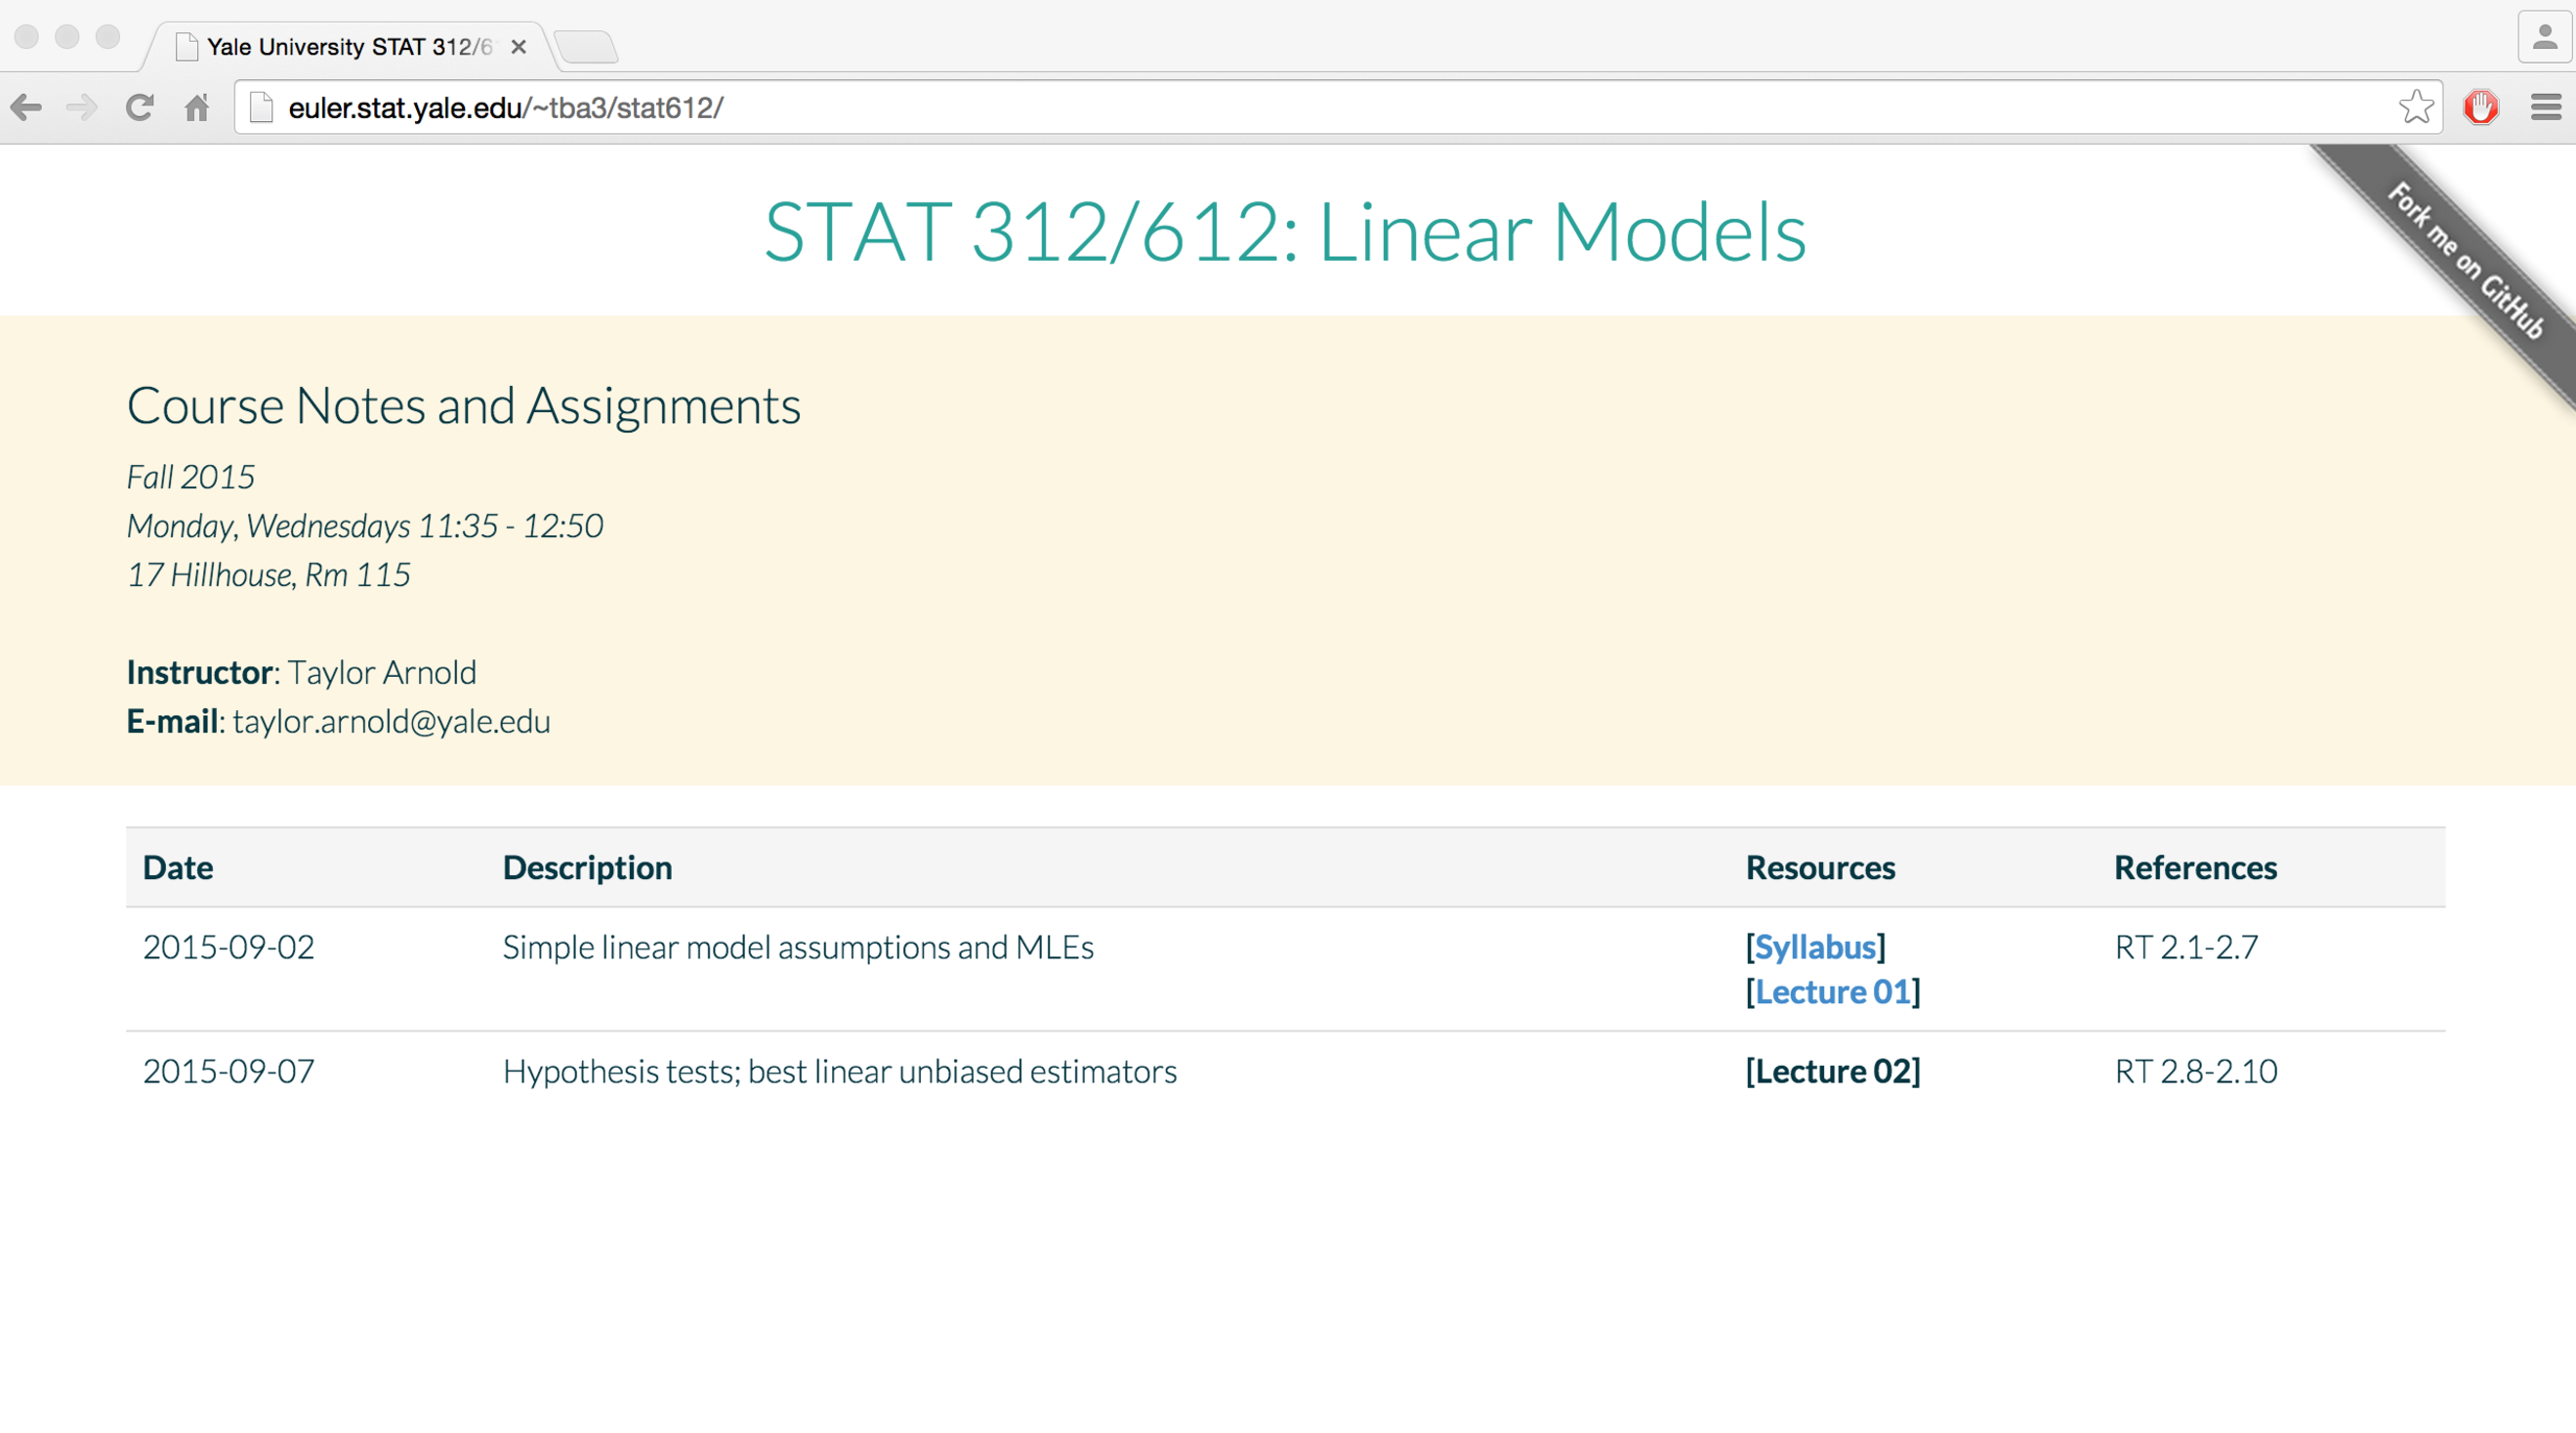
\includegraphics[width=\linewidth]{img/websiteScreenshot.pdf}

\end{frame}

%%%%%%%%%%%%%%%%%%%%%%%%%%%%%%%%%%%%%%%%%%%%%%%%%%%
\begin{frame}[fragile] \frametitle{}

\begin{flushright}
{\color{yaleblue}\sc\fontsize{1cm}{0cm}\selectfont Texts}
\end{flushright}

\end{frame}

%%%%%%%%%%%%%%%%%%%%%%%%%%%%%%%%%%%%%%%%%%%%%%%%%%%
\begin{frame}[fragile] \frametitle{}

\noindent
\begin{minipage}{0.5\textwidth}
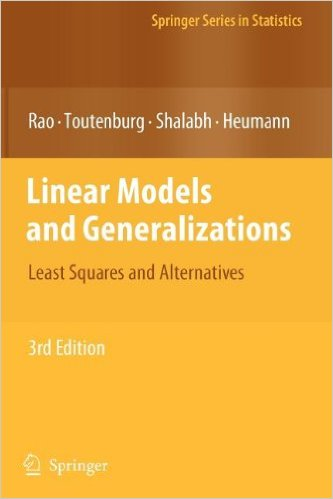
\includegraphics[width=0.9\linewidth]{img/rao.jpg}
\end{minipage}%%% to prevent a space
\begin{minipage}{0.5\textwidth}
Rao, Calyampudi R., et al. {\it Linear models}. Springer New York, 2008. \\
\begin{itemize}
\item Available digitally through Springer Link (free pdfs from Yale network)
\item Solid all-around reference on linear models
\item Many special cases and extensions; will be a source of many problem set questions
\end{itemize}
\end{minipage}

\end{frame}

%%%%%%%%%%%%%%%%%%%%%%%%%%%%%%%%%%%%%%%%%%%%%%%%%%%
\begin{frame}[fragile] \frametitle{}

\noindent
\begin{minipage}{0.5\textwidth}
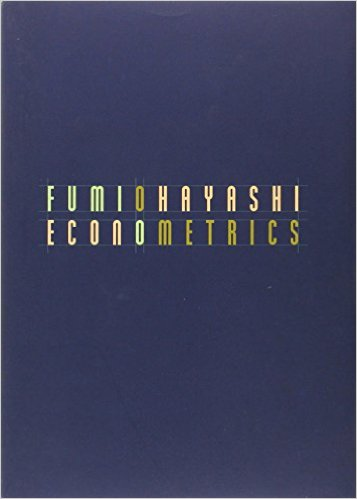
\includegraphics[width=0.9\linewidth]{img/hayashi.jpg}
\end{minipage}%%% to prevent a space
\begin{minipage}{0.5\textwidth}
Hayashi, Fumio. {\it Econometrics}. Princeton University Press. (2000). \\
\begin{itemize}
\item My go-to reference for multivariate regression results and notation
\item Intended for econometrics audience, but very thorough and theoretically sound
\item Will primarily look at first two chapters only
\item Focused on random design (stochastic X) and GMM methods
\item Intro chapter available from publisher as a free pdf
\end{itemize}
\end{minipage}

\end{frame}

%%%%%%%%%%%%%%%%%%%%%%%%%%%%%%%%%%%%%%%%%%%%%%%%%%%
\begin{frame}[fragile] \frametitle{}

\noindent
\begin{minipage}{0.5\textwidth}

\includegraphics[width=0.9\linewidth]{img/golub.jpg}
\end{minipage}%%% to prevent a space
\begin{minipage}{0.5\textwidth}
Golub, Gene H., and Charles F. Van Loan. {\it Matrix computations}. Vol. 3. JHU Press, 2012. \\
\begin{itemize}
\item Considered the canonical reference on numerical linear algebra
\item Not easily available online
\item Will quickly go through the chapter on least squares estimators
\end{itemize}
\end{minipage}

\end{frame}

%%%%%%%%%%%%%%%%%%%%%%%%%%%%%%%%%%%%%%%%%%%%%%%%%%%
\begin{frame}[fragile] \frametitle{}

\noindent
\begin{minipage}{0.5\textwidth}
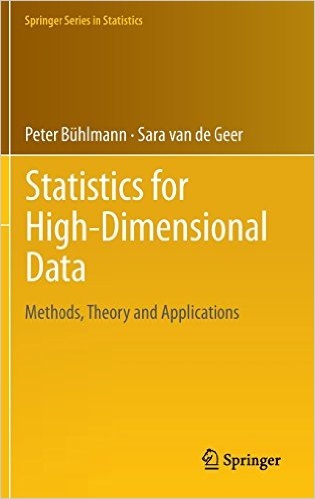
\includegraphics[width=0.9\linewidth]{img/buhlmann.jpg}
\end{minipage}%%% to prevent a space
\begin{minipage}{0.5\textwidth}
Bühlmann, Peter, and Sara Van De Geer. {\it Statistics for high-dimensional data: methods, theory and applications}. Springer Science \& Business Media, 2011. \\
\begin{itemize}
\item Available digitally through Springer Link (free pdfs from Yale network)
\item A good reference for $\ell_1$-penalized estimation
\item Ignoring first $100$ pages, gives a very thorough grounding on the basic theory and extensions
\item Will reference this a lot when we study penalized estimators
\end{itemize}
\end{minipage}
\end{frame}



%%%%%%%%%%%%%%%%%%%%%%%%%%%%%%%%%%%%%%%%%%%%%%%%%%%
\begin{frame}[fragile] \frametitle{}

\begin{flushright}
{\color{yaleblue}\sc\fontsize{1cm}{0cm}\selectfont Me!}
\end{flushright}

\end{frame}

%%%%%%%%%%%%%%%%%%%%%%%%%%%%%%%%%%%%%%%%%%%%%%%%%%%
\begin{frame}[fragile] \frametitle{}

\noindent
\begin{minipage}{0.4\textwidth}
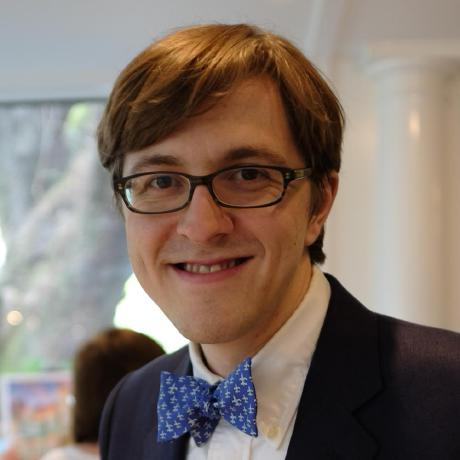
\includegraphics[width=0.9\linewidth]{img/arnold.jpeg}
\end{minipage}%%% to prevent a space
\begin{minipage}{0.6\textwidth}
Joint appointment at Yale Statistics and AT\&T Labs Research
\begin{itemize}
\item Research focus on large-scale data analysis (think, petabytes)
\item One focus is on encoding sparsity through penalized estimation
\item Applications to humanities and social sciences through with
analysis of image, text, and video corpora
\end{itemize}
\end{minipage}
\end{frame}

%%%%%%%%%%%%%%%%%%%%%%%%%%%%%%%%%%%%%%%%%%%%%%%%%%%
\begin{frame}[fragile] \frametitle{}

\begin{flushright}
{\color{yaleblue}\sc\fontsize{1cm}{1.2cm}\selectfont What exactly are \\\medskip Linear Models?}
\end{flushright}

\end{frame}

%%%%%%%%%%%%%%%%%%%%%%%%%%%%%%%%%%%%%%%%%%%%%%%%%%%
\begin{frame}[fragile] \frametitle{}

Consider observing pairs of points $(x_i,y_i)$, which we
can graphically represent by a scatter plot.

\vfill

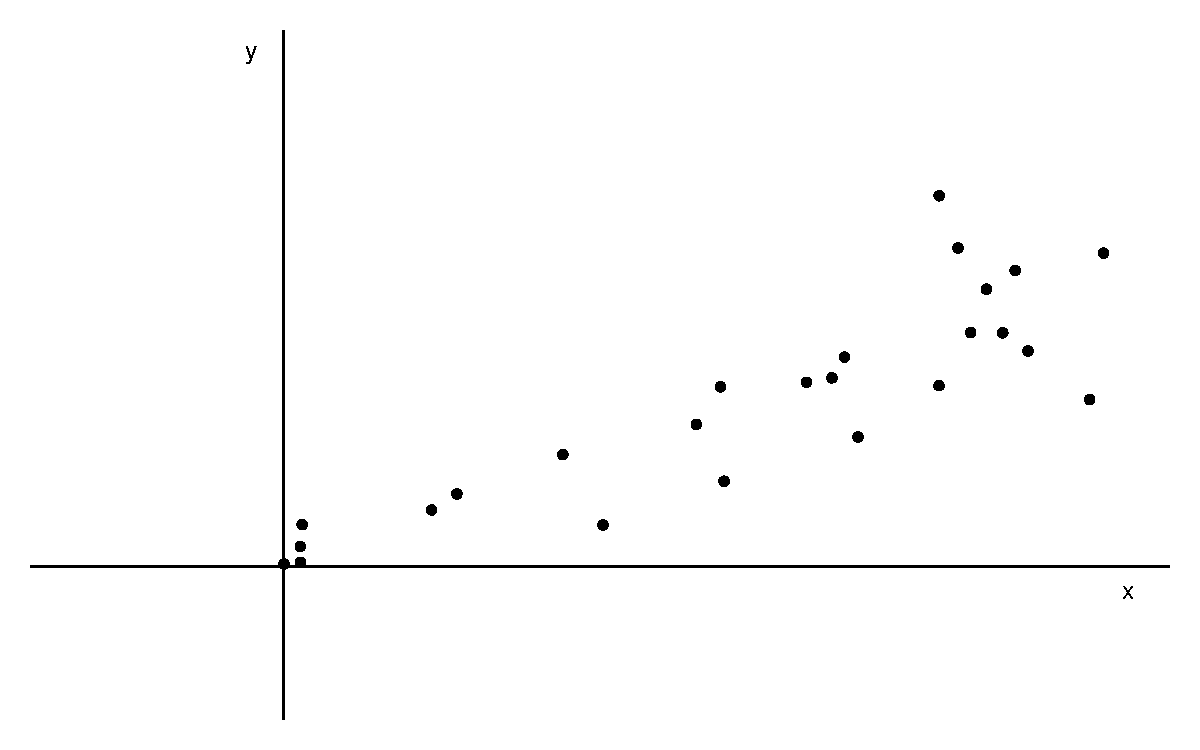
\includegraphics[width=0.9\linewidth]{img/fig01.pdf}

\end{frame}

%%%%%%%%%%%%%%%%%%%%%%%%%%%%%%%%%%%%%%%%%%%%%%%%%%%
\begin{frame}[fragile] \frametitle{}

A {\bf simple linear model} assumes that the mean of each
$y_i$ conditioned on $x_i$ is a linear function of $x_i$.

\vfill

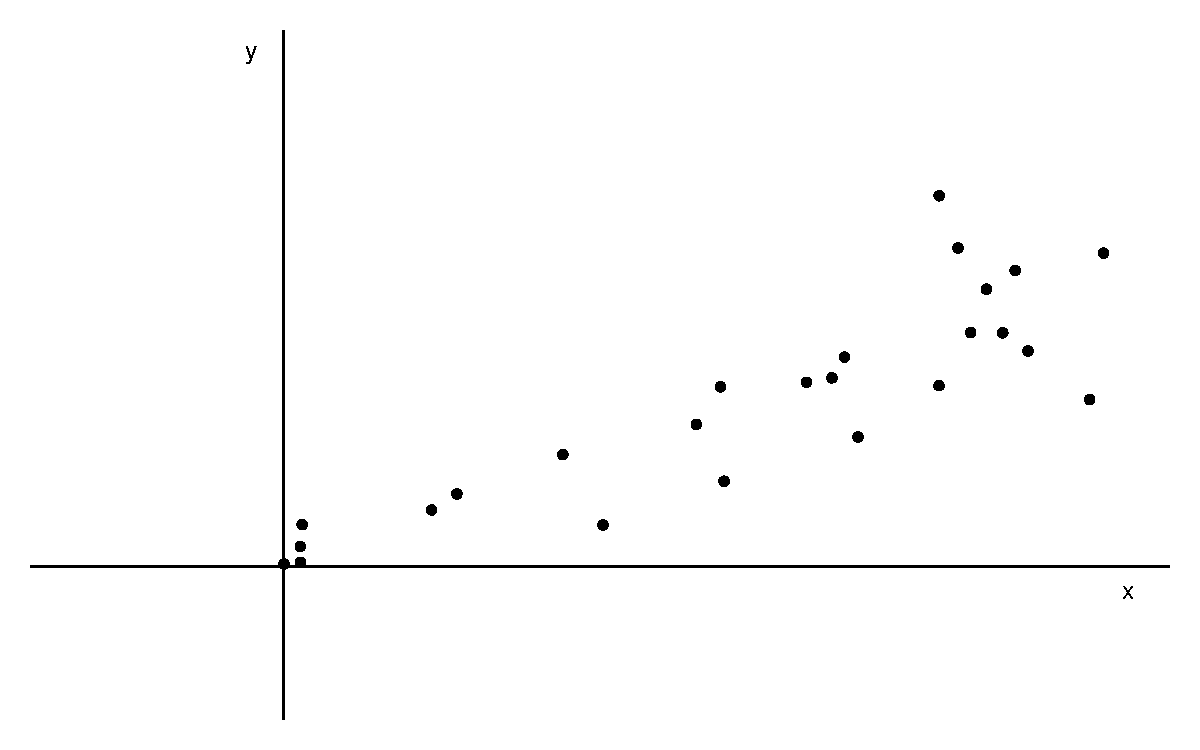
\includegraphics[width=0.9\linewidth]{img/fig01.pdf}

\end{frame}

%%%%%%%%%%%%%%%%%%%%%%%%%%%%%%%%%%%%%%%%%%%%%%%%%%%
\begin{frame}[fragile] \frametitle{}

Visually, we can think of this as a line through the data.

\vfill

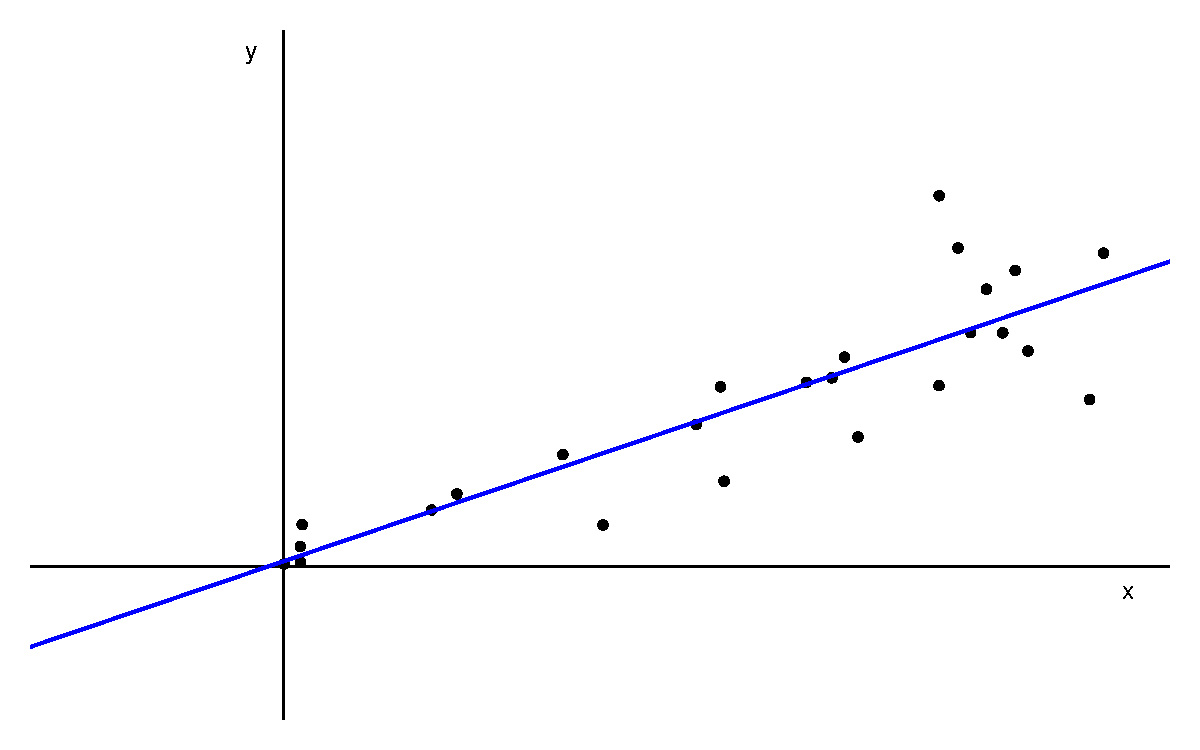
\includegraphics[width=0.9\linewidth]{img/fig02.pdf}

\end{frame}

%%%%%%%%%%%%%%%%%%%%%%%%%%%%%%%%%%%%%%%%%%%%%%%%%%%
\begin{frame}[fragile] \frametitle{}

For a reasonable fit, the {\bf residuals}, shown in red,
should have a mean close to zero. The should also be `small'
in some sense.

\vfill

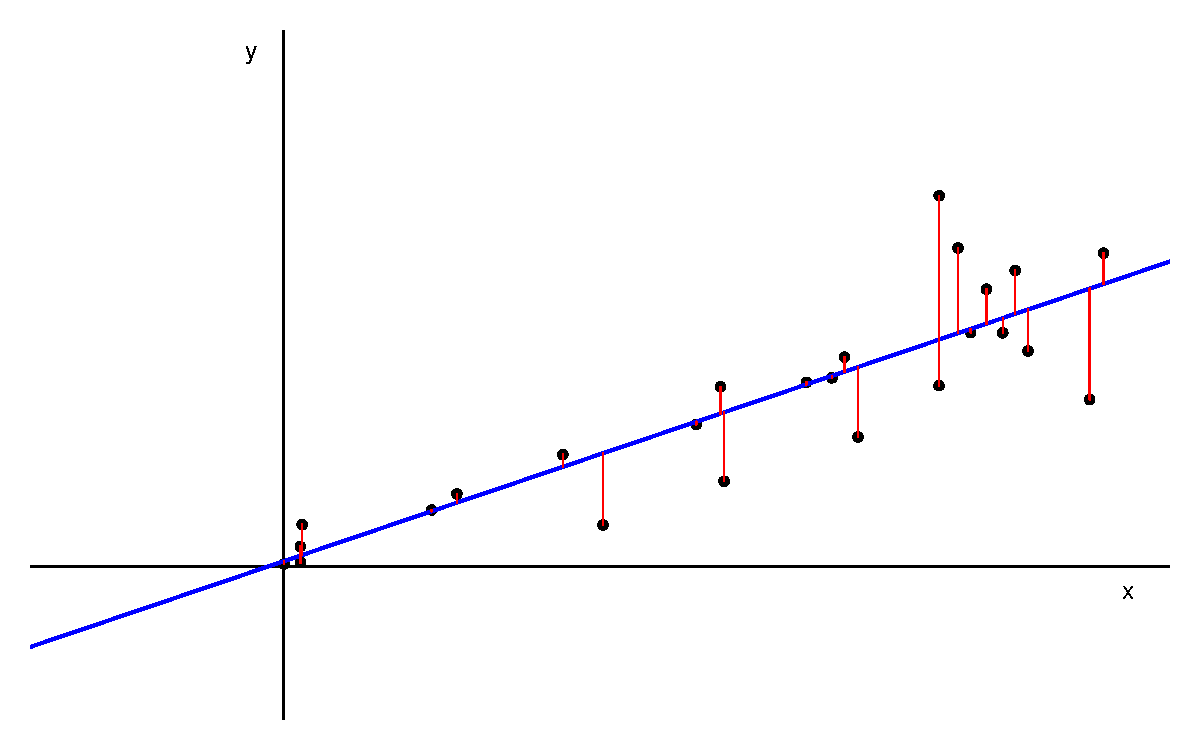
\includegraphics[width=0.9\linewidth]{img/fig03.pdf}

\end{frame}

%%%%%%%%%%%%%%%%%%%%%%%%%%%%%%%%%%%%%%%%%%%%%%%%%%%
\begin{frame}[fragile] \frametitle{}

Symbolically, the simple linear regression model assumes
that:
\begin{align}
\mathbb{E}(y_i|x_i) &= \alpha + x_i \cdot \beta
\end{align}
The goal, typically, is to find point estimates and conduct
inference on the unknown parameters $\alpha$ and $\beta$.

\end{frame}

%%%%%%%%%%%%%%%%%%%%%%%%%%%%%%%%%%%%%%%%%%%%%%%%%%%
\begin{frame}[fragile] \frametitle{}

Classic examples of quantities modelled with simple linear regression:
\begin{itemize}
\item College GPA $\sim$ SAT scores
\item Change in GDP $\sim$ change in unemployment
\item House price $\sim$ number of bedrooms
\item Species heart weight $\sim$ species body weight
\item Fatilities per year $\sim$ speed limit
\end{itemize}

\pause
Notice that these simple linear regressions are simplifications of
more complex relationships between the variables in question.

\end{frame}

%%%%%%%%%%%%%%%%%%%%%%%%%%%%%%%%%%%%%%%%%%%%%%%%%%%
\begin{frame}[fragile] \frametitle{}

What sign would be expect of $\beta$ (the slope) from
each of these?
\begin{itemize}
\item College GPA $\sim$ SAT scores \pause  $\quad{\color{solarized@green} \beta > 0}$
\item Change in GDP $\sim$ change in unemployment \pause $\quad{\color{solarized@red}\beta < 0}$
\item House price $\sim$ number of bedrooms \pause $\quad{\color{solarized@green}\beta > 0}$
\item Species heart weight $\sim$ species body weight \pause $\quad{\color{solarized@green}\beta > 0}$
\item Fatilities per year $\sim$ speed limit \pause $\quad{\color{solarized@red}\beta < 0}$
\end{itemize}

\end{frame}

%%%%%%%%%%%%%%%%%%%%%%%%%%%%%%%%%%%%%%%%%%%%%%%%%%%
\begin{frame}[fragile] \frametitle{}

A {\bf (general) linear model} is similiar to the simple variant, but
with a multivariate $x \in \mathbb{R}^p$ and a mean given by a hyperplane
in place of a single line.
\begin{align}
\mathbb{E}(y_i|x_i) &= \alpha + \sum_j \quad x_{i,j} \cdot \beta_j
\end{align}

\end{frame}

%%%%%%%%%%%%%%%%%%%%%%%%%%%%%%%%%%%%%%%%%%%%%%%%%%%
\begin{frame}[fragile] \frametitle{}


\begin{itemize}
\item General principles are the same as the simple case \pause
\item Math is more difficult because we need to use matricies \pause
\item Interpretation is more difficult because the $\beta_j$ are effects
conditional on the other variables
\end{itemize}

\end{frame}


%%%%%%%%%%%%%%%%%%%%%%%%%%%%%%%%%%%%%%%%%%%%%%%%%%%
\begin{frame}[fragile] \frametitle{}

For example, consider these two variable regressions:
\begin{itemize}
\item College GPA $\sim$ SAT scores, secondary school GPA
\item Change in GDP $\sim$ change in unemployment, inflation
\item House price $\sim$ number of bedrooms, area of the house
\item Species heart weight $\sim$ species body weight, species height
\item Fatilities per year $\sim$ speed limit, minimum legal speed
\end{itemize}

\pause
Many would retain the same signs as the simple linear regression, but
the magnitudes would be smaller. In some cases, it is possible for
the relationship to flip directions when a second (highly correlated)
variable is added.

\end{frame}

%%%%%%%%%%%%%%%%%%%%%%%%%%%%%%%%%%%%%%%%%%%%%%%%%%%
\begin{frame}[fragile] \frametitle{}

What might be an explanation of the following signs:
\begin{itemize}
\item College GPA $\sim$ {\color{solarized@red} SAT scores}, {\color{solarized@green} secondary school GPA} \pause
\item House price $\sim$ {\color{solarized@green} number of bedrooms},
      {\color{solarized@red} area of the house} \pause
\item Species heart weight $\sim$ {\color{solarized@green} species body weight}, {\color{solarized@red} species height}
\end{itemize}

\end{frame}


%%%%%%%%%%%%%%%%%%%%%%%%%%%%%%%%%%%%%%%%%%%%%%%%%%%
\begin{frame}[fragile] \frametitle{}

Extensions to linear models include: \pause
\begin{itemize} \setlength\itemsep{0em}
\item generalized linear models:
\begin{align*}
\mathbb{E} (y | x) &= g^{-1}(x^t \beta)
\end{align*} \pause
\item additive models:
\begin{align*}
\mathbb{E} (y | x) &= f_1(x_1) + f_2(x_2) + \cdots + f_k(x_k)
\end{align*} \pause
\item Generalized Additive Model for Location, Scale and Shape (GAMLSS):
\begin{align*}
\mathbb{E} (y | x) &= f_{1,1}(x_1) + f_{1,1}(x_2) + \cdots + f_{1,1}(x_k) \\
\mathbb{E} (y^2 | x) &= f_{1,2}(x_1) + f_{2,2}(x_2) + \cdots + f_{k,2}(x_k) \\
&\vdots \\
\mathbb{E} (y^q | x) &= f_{1,q}(x_1) + f_{2,q}(x_2) + \cdots + f_{k,q}(x_k) \\
\end{align*}
\end{itemize}

\end{frame}

%%%%%%%%%%%%%%%%%%%%%%%%%%%%%%%%%%%%%%%%%%%%%%%%%%%
\begin{frame}[fragile] \frametitle{}

\begin{flushright}
{\color{yaleblue}\sc\fontsize{1cm}{1cm}\selectfont Machine Learning \& \\\medskip Linear Models}
\end{flushright}

\end{frame}

%%%%%%%%%%%%%%%%%%%%%%%%%%%%%%%%%%%%%%%%%%%%%%%%%%%
\begin{frame}[fragile] \frametitle{}

Machine learning is a closely related field to statistics; most
researches that I know think of there being a spectrum of research
between the two rather than a clear dividing line. \pause

If forced to catagorize them, I would describe statistics as
being primarily concerned with {\bf inference} and machine learning
with {\bf prediction}.

\end{frame}

%%%%%%%%%%%%%%%%%%%%%%%%%%%%%%%%%%%%%%%%%%%%%%%%%%%
\begin{frame}[fragile] \frametitle{}

{\color{yaleblue}\fontsize{16pt}{20pt}\selectfont Question}

With powerful methods such as neural networks, support vector
machines, and gradient boosted trees, is there space for
linear models in machine learning?

\end{frame}

%%%%%%%%%%%%%%%%%%%%%%%%%%%%%%%%%%%%%%%%%%%%%%%%%%%
\begin{frame}[fragile] \frametitle{}

{\color{yaleblue}\fontsize{16pt}{20pt}\selectfont Answer}

Yes!

\end{frame}

%%%%%%%%%%%%%%%%%%%%%%%%%%%%%%%%%%%%%%%%%%%%%%%%%%%
\begin{frame}[fragile] \frametitle{}

{\bf \# 1.} When the number of parameters is close to or exceeds the
number of observations, particularly if the data matrix $X$ is sparse.

\end{frame}

%%%%%%%%%%%%%%%%%%%%%%%%%%%%%%%%%%%%%%%%%%%%%%%%%%%
\begin{frame}[fragile] \frametitle{}

{\bf \# 2.} Creating meta-variables as an input to other ML techniques
or to blend the outputs from ensemble learning.

\end{frame}

%%%%%%%%%%%%%%%%%%%%%%%%%%%%%%%%%%%%%%%%%%%%%%%%%%%
\begin{frame}[fragile] \frametitle{}

{\bf \# 3.} Working with data that have difficult to
work with distributions, such as quantile regression on
heavy-tailed errors (i.e., Cauchy, Lévy).

\end{frame}

%%%%%%%%%%%%%%%%%%%%%%%%%%%%%%%%%%%%%%%%%%%%%%%%%%%
\begin{frame}[fragile] \frametitle{}

{\bf \# 4.} Projecting into high dimensional spaces (where often
we have more predictors that observations and spare data matrices).

\end{frame}

%%%%%%%%%%%%%%%%%%%%%%%%%%%%%%%%%%%%%%%%%%%%%%%%%%%
\begin{frame}[fragile] \frametitle{}

\begin{flushright}
{\color{yaleblue}\sc\fontsize{1cm}{1cm}\selectfont When `Linear' \\\medskip Isn't}
\end{flushright}

\end{frame}

%%%%%%%%%%%%%%%%%%%%%%%%%%%%%%%%%%%%%%%%%%%%%%%%%%%
\begin{frame}[fragile] \frametitle{}

Consider the following set of data points $(x_i, y_i)$. The relationship
between $x$ and $y$ is highly non-linear.

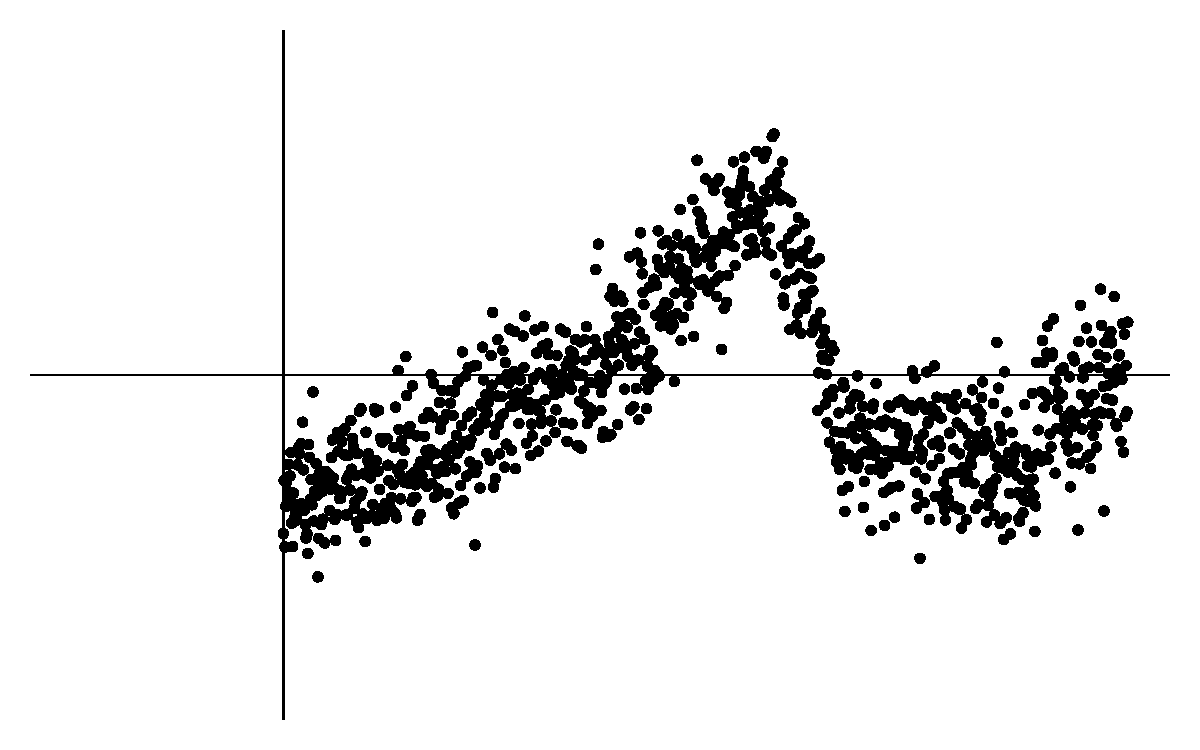
\includegraphics[width=\linewidth]{img/fig04.pdf}

\end{frame}

%%%%%%%%%%%%%%%%%%%%%%%%%%%%%%%%%%%%%%%%%%%%%%%%%%%
\begin{frame}[fragile] \frametitle{}

The true mean (from which I simulated) is given by:

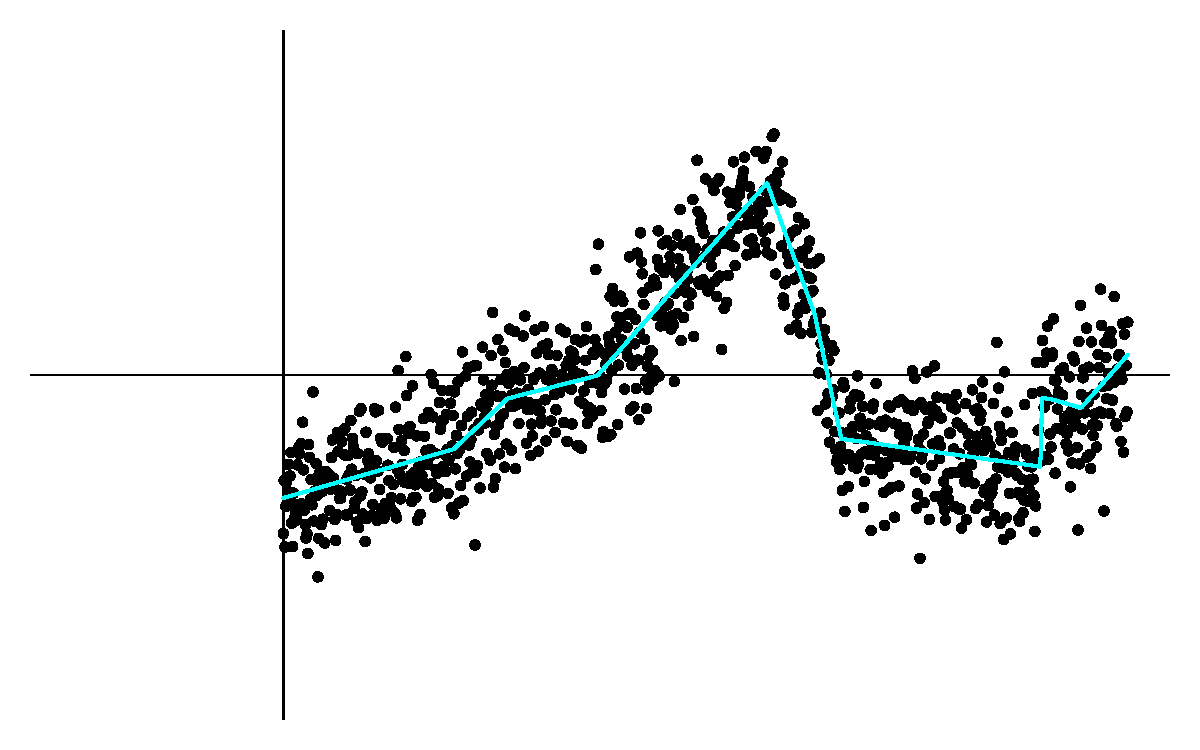
\includegraphics[width=\linewidth]{img/fig05.pdf}

\end{frame}

%%%%%%%%%%%%%%%%%%%%%%%%%%%%%%%%%%%%%%%%%%%%%%%%%%%
\begin{frame}[fragile] \frametitle{}

It would at first seem that we can't model this response with a linear
model. However, that is not the case because it is only $\beta$ that needs to be
linear, not the $x$ values. \pause

For example, the following is a linear model:
\begin{align*}
\mathbb{E} (y | x) &= \beta_0 + \beta_1 x^1 + \beta_2 x^2 + \beta_3 x^3
\end{align*}
Which will fit a polynomial to the data.

\end{frame}

%%%%%%%%%%%%%%%%%%%%%%%%%%%%%%%%%%%%%%%%%%%%%%%%%%%
\begin{frame}[fragile] \frametitle{}

An alternative that works better here, is a Fourier basis:
\begin{align*}
\mathbb{E} (y | x) &= \beta_0 + \sum_{j=1}^{k} \beta_j \cos (j * x) + \sum_{j=1}^k \beta_{k+j} \sin (j * x)
\end{align*}
And we can adjust the fit appropriately by specifying the
order $k$.

\end{frame}


%%%%%%%%%%%%%%%%%%%%%%%%%%%%%%%%%%%%%%%%%%%%%%%%%%%
\begin{frame}[fragile] \frametitle{}

$k=1$

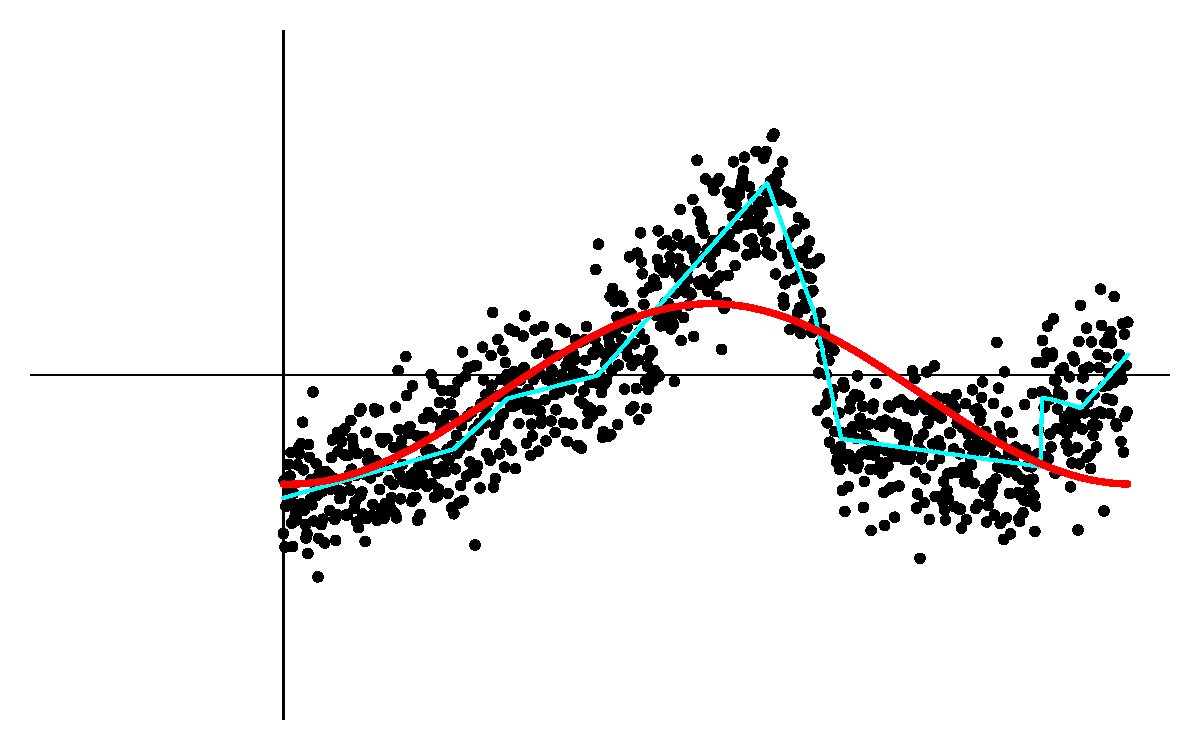
\includegraphics[width=\linewidth]{img/fig06.pdf}

\end{frame}


%%%%%%%%%%%%%%%%%%%%%%%%%%%%%%%%%%%%%%%%%%%%%%%%%%%
\begin{frame}[fragile] \frametitle{}

$k=2$

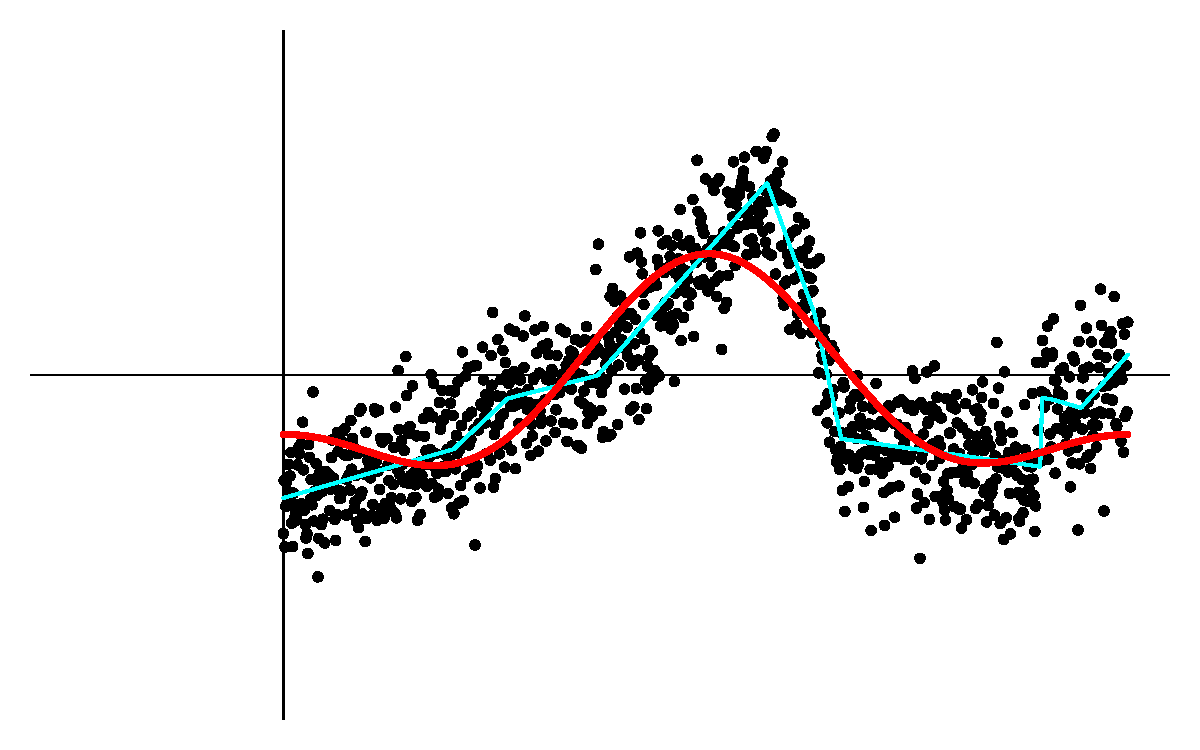
\includegraphics[width=\linewidth]{img/fig07.pdf}

\end{frame}


%%%%%%%%%%%%%%%%%%%%%%%%%%%%%%%%%%%%%%%%%%%%%%%%%%%
\begin{frame}[fragile] \frametitle{}

$k=3$

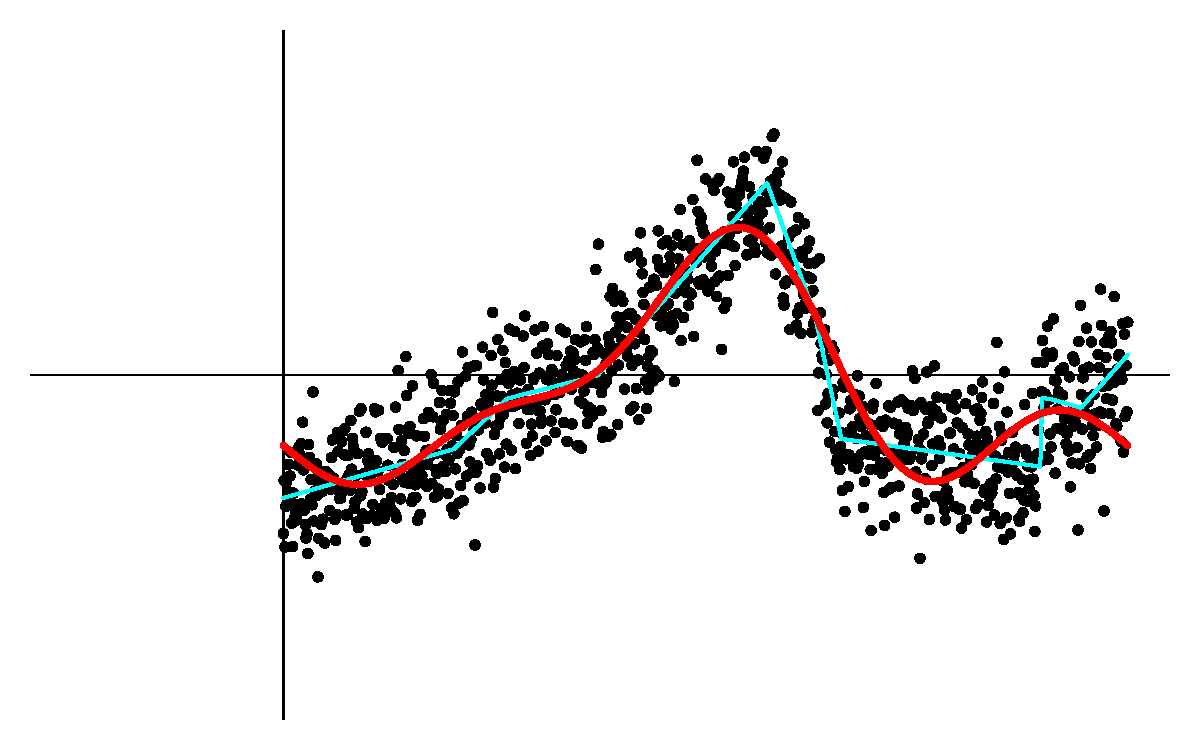
\includegraphics[width=\linewidth]{img/fig08.pdf}

\end{frame}


%%%%%%%%%%%%%%%%%%%%%%%%%%%%%%%%%%%%%%%%%%%%%%%%%%%
\begin{frame}[fragile] \frametitle{}

$k=4$

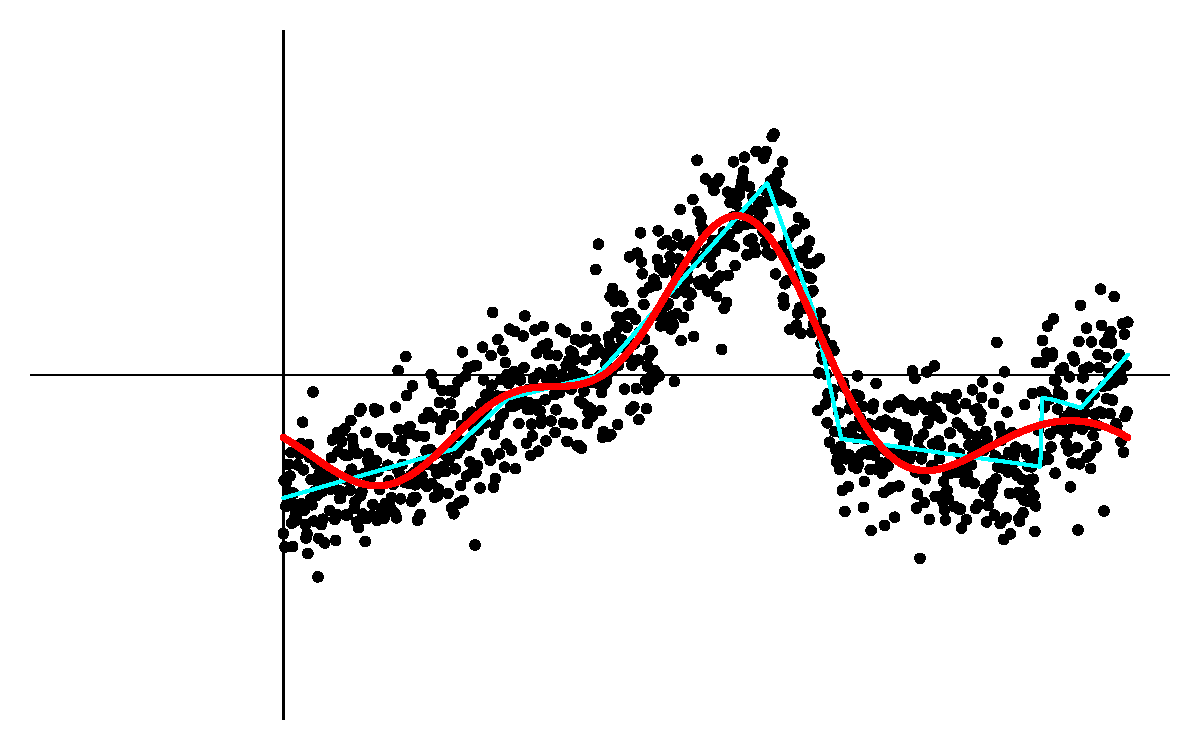
\includegraphics[width=\linewidth]{img/fig09.pdf}

\end{frame}

%%%%%%%%%%%%%%%%%%%%%%%%%%%%%%%%%%%%%%%%%%%%%%%%%%%
\begin{frame}[fragile] \frametitle{}

$k=20$

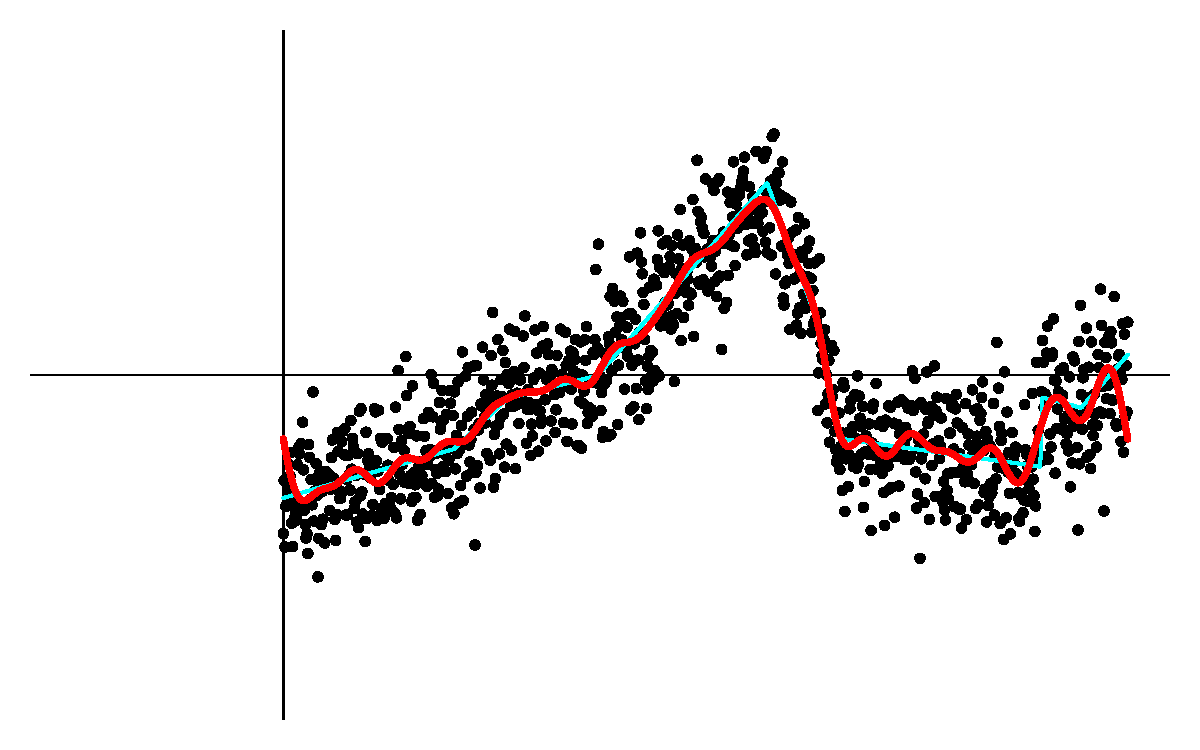
\includegraphics[width=\linewidth]{img/fig10.pdf}

\end{frame}

%%%%%%%%%%%%%%%%%%%%%%%%%%%%%%%%%%%%%%%%%%%%%%%%%%%
\begin{frame}[fragile] \frametitle{}

{\color{yaleblue}\fontsize{16pt}{20pt}\selectfont Questions, thoughts or concerns?} \pause

website: \url{http://euler.stat.yale.edu/~tba3/stat612} \\
e-mail: {\tt taylor.arnold{@}yale.edu}


\end{frame}


\end{document}













